
\subsection{Ordnung}
\begin{frame}[t]{Dateien ordentlich ablegen}
    \begin{columns}
        \begin{column}{0.5\textwidth}
            \vspace{-6cm}
            \begin{block}{Ein paar Grundregeln}
                \begin{itemize}
                    \item Überlegt euch eine Struktur.                 
                    \item Versucht möglichst wenige Ordner Level zu haben.
                    \item Schreibt eure Struktur auf. Gute Angewohnheit: Eine ReadMe in den Top Ordner legen.
            \end{itemize}  
            \end{block}
            {\small Ein paar Quellen:
            \begin{itemize}[]
                \item \href{https://www.youtube.com/watch?v=WtKeeDYA_2I&t=317s}{YouTube}
                \item \href{https://ocw.mit.edu/courses/res-str-002-data-management-spring-2016/497580bd31c004cc758a2afb0a115aa4_MITRES_STR_002S16_File.pdf}{MIT Open Courseware}
            \end{itemize}
            }

            \vfill   
        \end{column}
        \begin{column}[t]{0.5\textwidth}
            \begin{forest}
                for tree={
                    font=\ttfamily,
                    grow'=0,
                    child anchor=west,
                    parent anchor=south,
                    anchor=west,
                    calign=first,
                    inner xsep=7pt,
                    s sep=1pt,
                    edge path={
                    \noexpand\path [draw, \forestoption{edge}]
                    (!u.south west) +(2pt,0) |- (.child anchor) pic {folder} \forestoption{edge label};
                    },
                    file/.style={edge path={\noexpand\path [draw, \forestoption{edge}]
                    (!u.south west) +(7.5pt,0) |- (.child anchor) \forestoption{edge label};},
                    inner xsep=2pt,inner ysep=0pt,font=\small\ttfamily
                            },
                    before typesetting nodes={
                    if n=1
                        {insert before={[,phantom]}}
                        {if n=3 
                        {insert before={[,phantom]}}
                        {}
                        }                
                    },
                    fit=band,
                    before computing xy={l=15pt},
                }  
                [SS24
                    [ReadMe.txt,file]
                    [Grundlagen 1
                        [SW1
                            [VL.pdf,file]
                            [Übung.pdf,file]
                        ]
                        [SW2]
                    ]
                    [Nebenfach 1
                        [VL
                            [VL1.pdf,file]
                            [VL2.pdf,file]
                        ]
                        [Übungen
                            [Ü1.pdf,file]
                            [Ü2.pdf,file]
                        ]
                    ]
                ]
                \end{forest}
        \end{column}
    \end{columns}
\end{frame}

\subsection{Zeitmanagement}

\begin{frame}{Stundenplan}
    \begin{figure}
       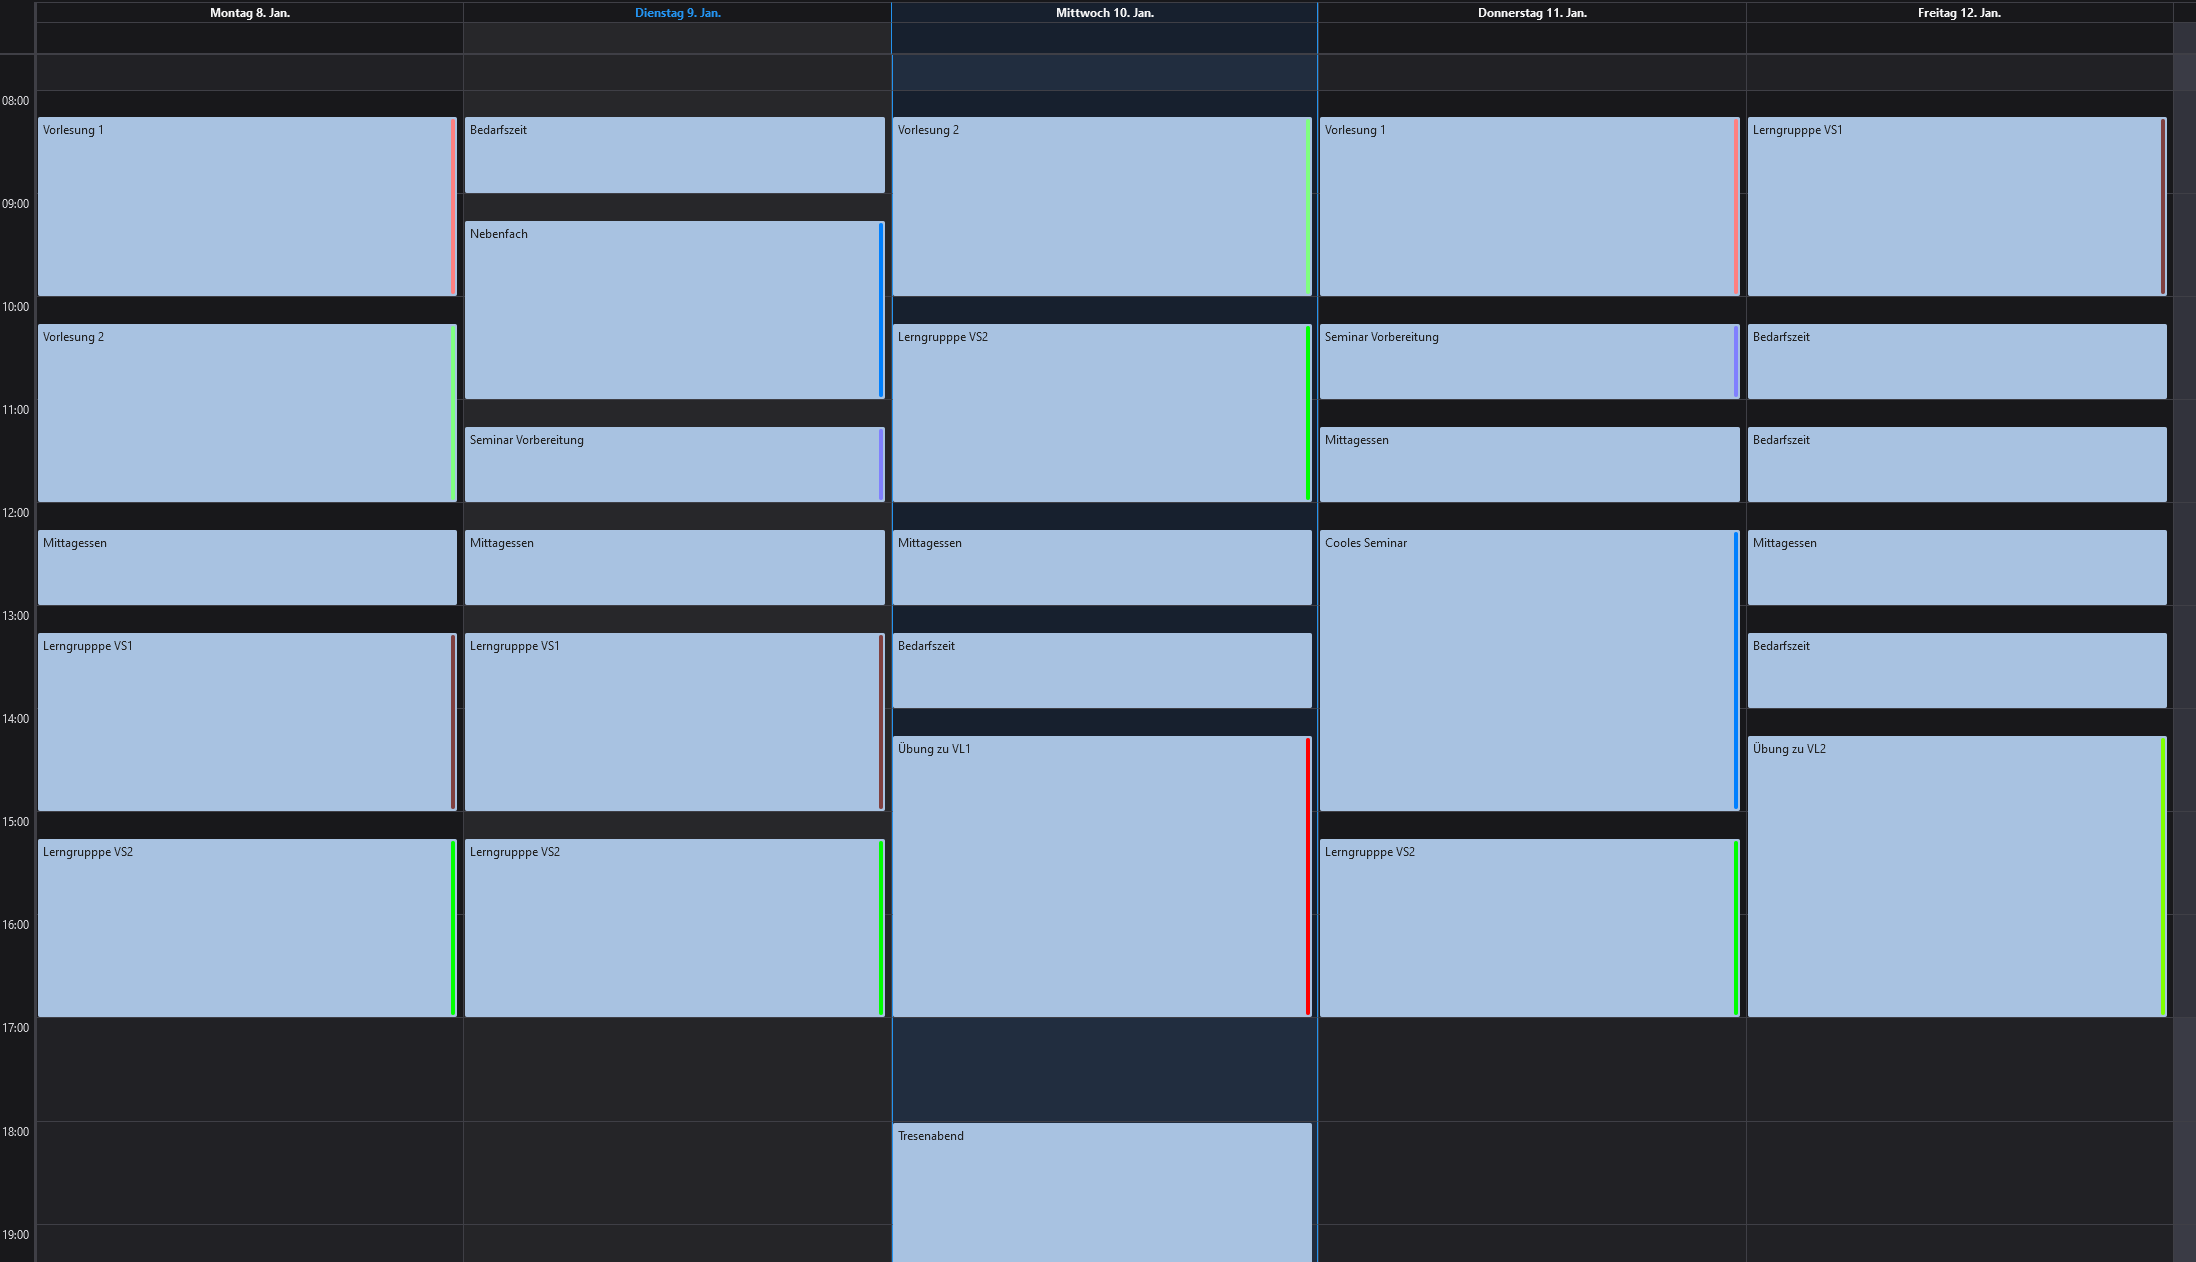
\includegraphics[width=0.8\textwidth]{graphics/Kalender/Kalender5.PNG};
    \end{figure}
\end{frame}

\begin{frame}{Time Boxing}    
    \begin{figure}
       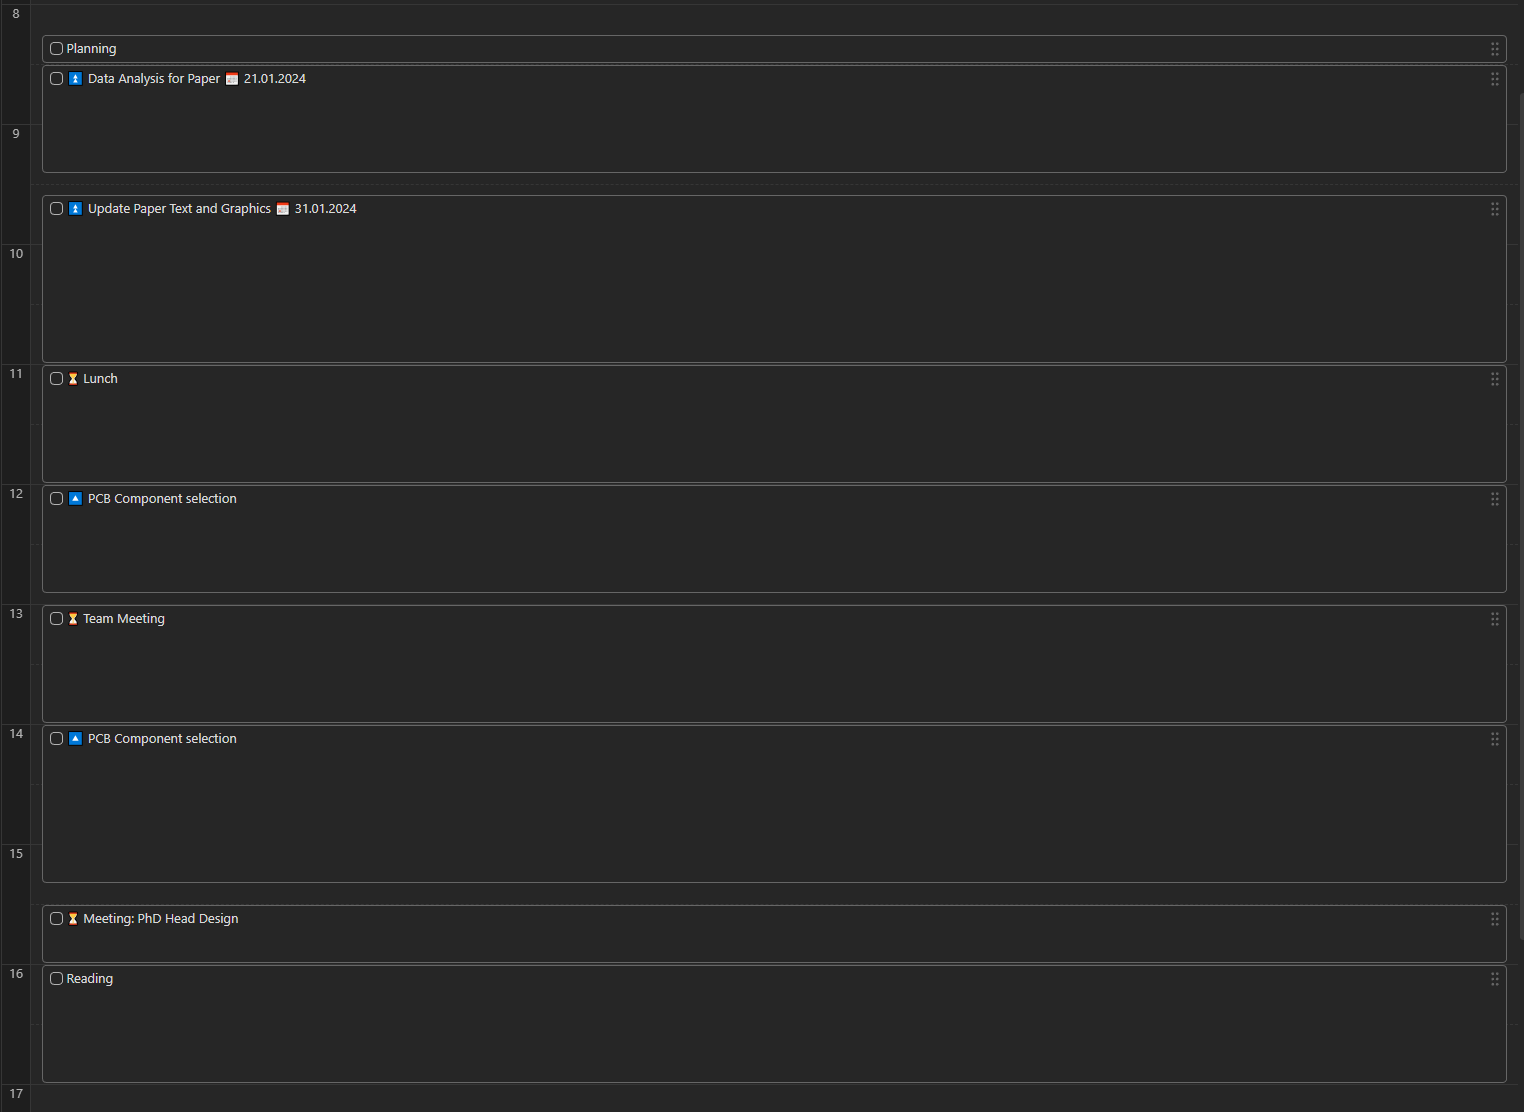
\includegraphics[height=0.8\textheight,trim={0 0 10cm 0},clip]{graphics/MyDailyPlan.png};
    \end{figure}
\end{frame}
\note{
Kalender       
Pomodoro}

\begin{frame}{Mehr Ansätze:}
    \begin{columns}[t]
        \begin{column}{0.3\textwidth}
            \begin{figure}
                \begin{flushleft}
                    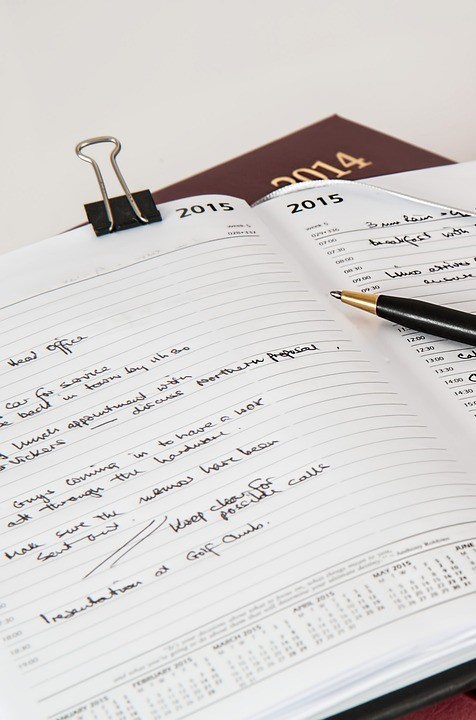
\includegraphics[width=\textwidth]{graphics/diary-614149_960_720.jpg}
                    \caption*{\href{https://pixabay.com/de/photos/tagebuch-stift-notizbuch-januar-614149/}{stevepb on pixabay}}    
                \end{flushleft}                
            \end{figure}
            
        \end{column}
        \begin{column}{0.7\textwidth}
            \begin{itemize}
                \item ToDo Listen
                \begin{itemize}
                    \item \href{https://to-do.office.com/tasks/}{Microsoft ToDo}
                    \item \href{https://todoist.com/de}{todoist}
                    \item \dots
                \end{itemize}
                \item Pomodoro Technik
                \item \begin{itemize}
                    \item \href{https://pomofocus.io/}{Pomofocus}
                    \item \dots
                \end{itemize}                 
            \end{itemize}
        \end{column}
    \end{columns}
\end{frame}


\begin{frame}{Und noch mehr}
    \begin{columns}[t]
    \begin{column}{0.49\textwidth}
        \begin{figure}
            \begin{flushleft}
                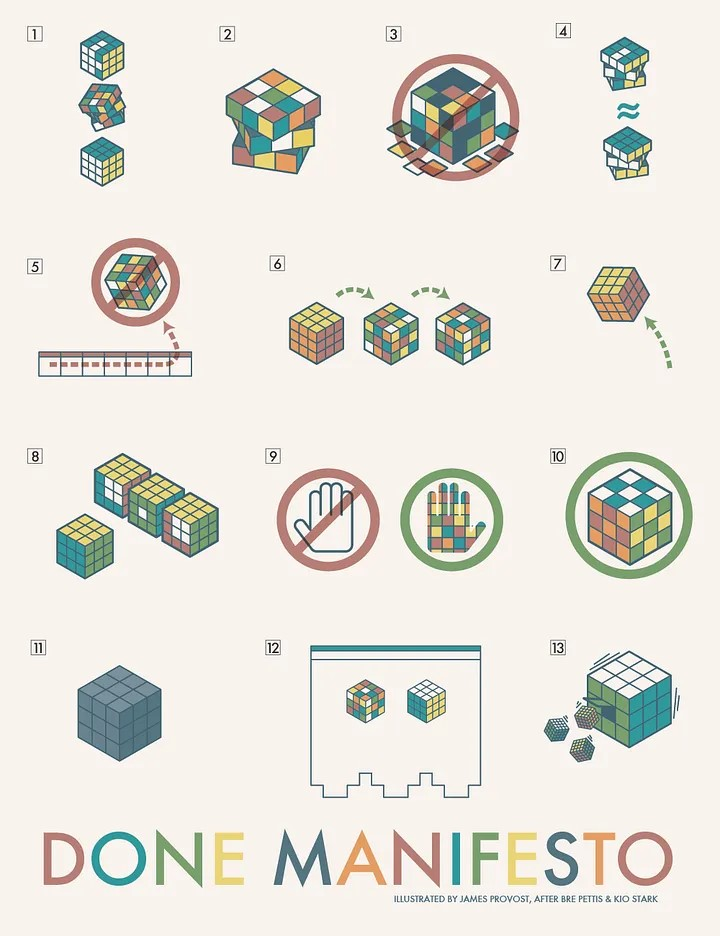
\includegraphics[height=0.7\textheight]{graphics/TheDoneManifesto.jpg}
                \caption*{\href{https://medium.com/@bre/the-cult-of-done-manifesto-724ca1c2ff13}{The Done Manifesto}}   
            \end{flushleft}                
        \end{figure}        
    \end{column}
    \begin{column}{0.49\textwidth}
        \begin{figure}
            \begin{flushleft}
                
\includegraphics[height=0.7\textheight]{graphics/GTD.png}
                \caption*{\href{https://www.thalia.de/shop/home/artikeldetails/A1052684525?ProvID=11000731&msclkid=add9b427aa0c13222c40d1b812e94a42&gclsrc=ds}{David Allen Getting Things Done}}    
            \end{flushleft}                
        \end{figure}        
    \end{column}
\end{columns}
\end{frame}